%!TEX root = draft.tex
\section{Queues With Fixed Dequeue Linearization Points}\label{sec:queues}

The typical abstract implementation of a concurrent queue, denoted by $AbsQ_0$, maintains a sequence of values, the enqueue method adds a value atomically to the beginning of the sequence, and the dequeue method removes a value from the end of the sequence (if any, otherwise it returns ``empty''). In this section, we describe another abstract implementation, denoted as $AbsQ$, which roughly maintains a \emph{partially-ordered set} of values instead of a sequence. We show that there exists a forward simulation from any correct queue implementation where the \emph{dequeue} methods have fixed linearization points (the enqueue methods are unconstrained) to $AbsQ$. This covers all the queue implementations that we are aware of. We describe a forward simulation from the Herlihy\&Wing queue~\cite{journals/toplas/HerlihyW90} to $AbsQ$.

\subsection{Abstract Queue Implementation}

Before describing our abstract implementation $AbsQ$, we present an example of a queue implementation where only the dequeue methods have fixed linearization points, namely the Herlihy \& Wing queue~\cite{journals/toplas/HerlihyW90} listed in Figure~\ref{fig:HerlihyWing} (we assume that every statement is atomic).

\begin{wrapfigure}{l}{5.7cm}
%\vspace{-8mm}
\begin{lstlisting}
void enq(int x){
  i = back++;
  items[i] = x;
}

int deq() {
  while (1) {
    range = back - 1;
    for (int i = 0; i <= range; i++){
      x = swap(items[i],null);
      if ( x != null ) return x;
    }
  }
}
  \end{lstlisting}
\vspace{-5mm}
\caption{Herlihy \& Wing queue.}
\label{fig:HerlihyWing}
\vspace{-6mm}
\end{wrapfigure}
The shared state consists of an array {\tt items} storing values in the queue and a counter {\tt back} storing the index of the first unused position in {\tt items}. Initially, all the positions in the array are {\tt null} and {\tt back} is 0.
An enqueue method starts by reserving a position in {\tt items} ({\tt i} stores the index of this position and {\tt back} is incremented so the same position can't be used by other enqueue operations) and then, storing the input value {\tt x} at this position. The dequeue method traverses the array {\tt items} starting from the beginning and atomically swaps {\tt null} with the encountered value. If the value is not {\tt null}, then the dequeue returns that value. If it reaches the end of the array, then it restarts.

The linearization points of the enqueue methods are not fixed, they depend on dequeue operations executing in the future. Consider the following trace with two concurrent enqueues (the local variables of operation $k$ are indexed by $k$):
\begin{align*}
inv(enq,x,1)\ \ \ inv(enq,y,2)\ \ \ {\tt i}_1 = \mbox{{\tt bck++}}\ \ \ {\tt i}_2 = \mbox{{\tt bck++}}\ \ \ {\tt items[i_2]} = y
\end{align*}
%\begin{align*}
%inv(enq,x,1)\ inv(enq,y,2)\ ({\tt i}_1 = 0,{\tt bck} = 1)\ ({\tt i}_2 = 1,{\tt bck} = 2)\ ({\tt items[1]} = y)
%\end{align*}
Assuming that the linearization point corresponds to the assignment of {\tt i}, the history of this trace should be linearized to $inv(enq,x,1)\ ret(enq,1)\ inv(enq,y,2)\ ret(enq,2)$. However, a dequeue operation executing until completion after this trace will return value $y$ (only position $1$ is filled in the array {\tt items}) which is not consistent with this linearization. On the other hand, assuming that enqueues should be linearized at the assignment of {\tt items[i]} and extending the trace with ${\tt items[i_1]} = x$ and a completed dequeue that in this case returns $x$, leads to an incorrect linearization 
\begin{align*}
inv(enq,y,2)\ ret(enq,2) inv(enq,x,1)\ ret(enq,1)\ inv(deq,3)\ ret(deq,1,3).
\end{align*}

The dequeue method has a fixed linearization point which corresponds to an execution of {\tt swap} returning a non-null value. This action alone contributes to the effect of that value being removed from the queue. This claim will be formally proved in Section~\ref{ssec:HerlihyWing}.

Since the linearization points of the enqueues are not fixed, it is not possible to define a forward simulation from the Herlihy \& Wing queue to the standard abstract implementation $AbsQ_0$. In the following, we describe the abstract implementation $AbsQ$ we propose for which such a forward simulation does exist.

Informally, $AbsQ$ records the happens-before order between enqueue operations for which the added value has not been removed by a dequeue operation. The linearization point of a dequeue operation with return value $d\neq{\tt EMPTY}$ is enabled only if the happens-before order stored in the current state contains a minimal enqueue operation that adds the value $d$. The effect of the linearization point is that the minimal enqueue is removed from the current state and the return value is recorded in the library state. When the return value is {\tt EMPTY}, the linearization point of a dequeue is enabled only if the current state stores no enqueue operation. The return of a dequeue is enabled only if the returned value matches the one fixed at the linearization point.

\begin{wrapfigure}{l}{7cm}
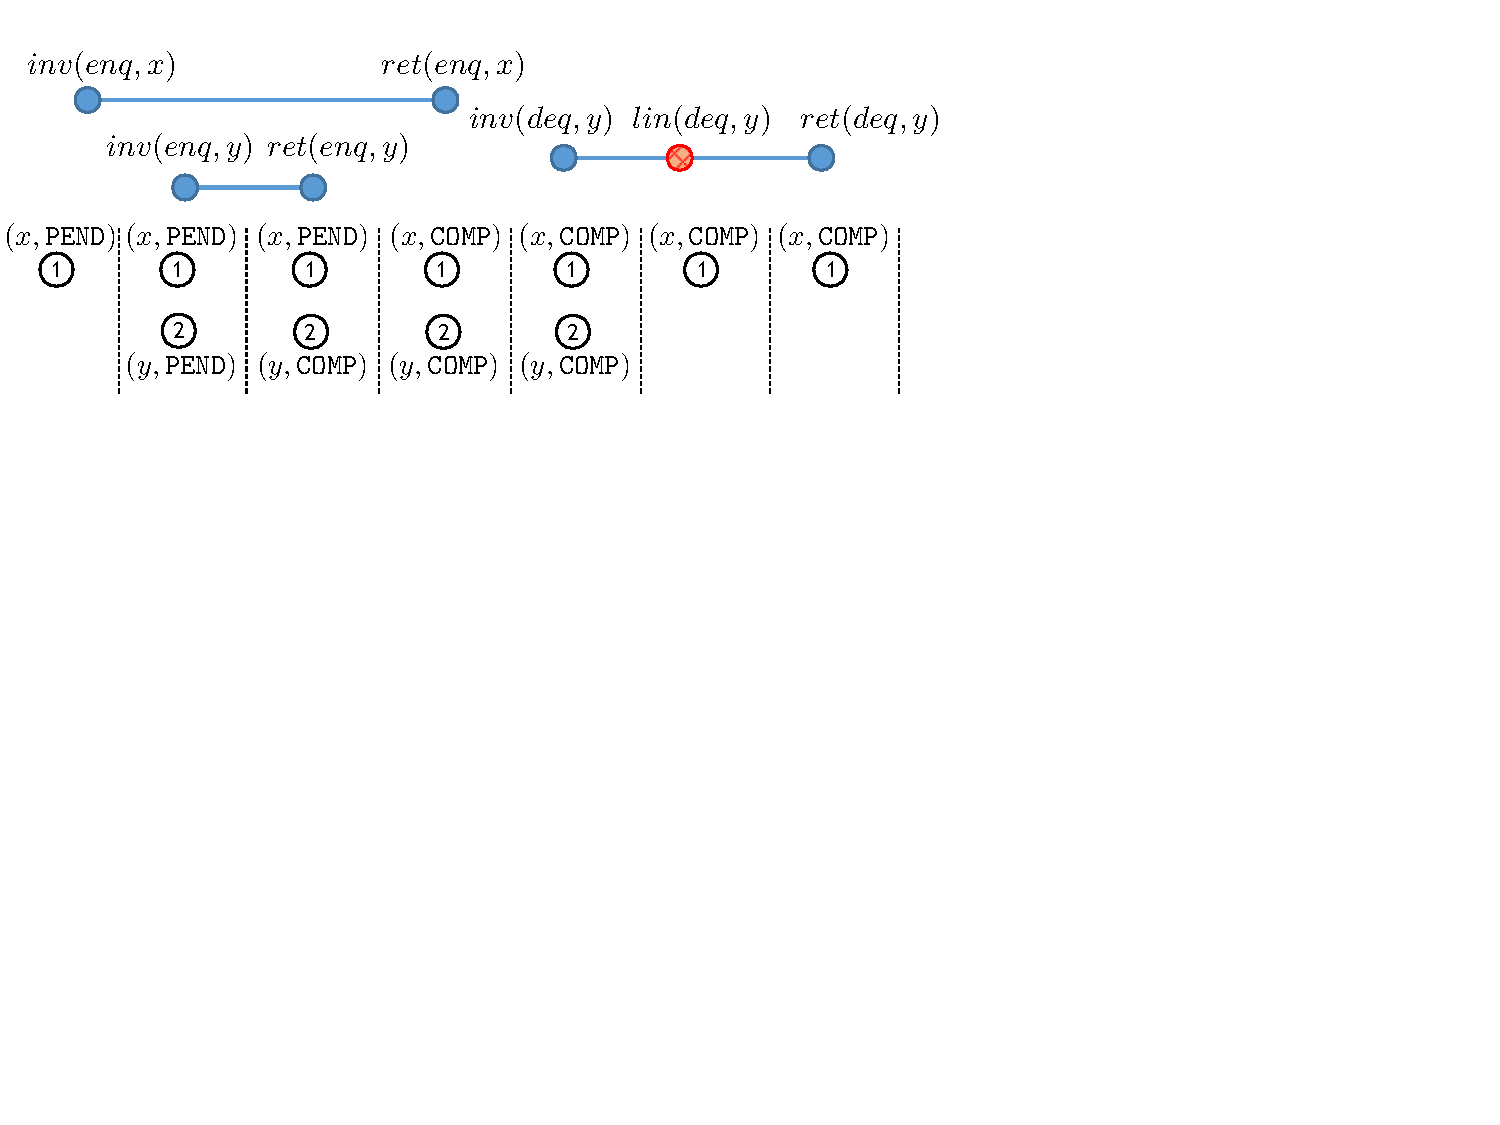
\includegraphics[width=7cm]{fig-queue1.pdf}
\begin{center}
(a)
\end{center}

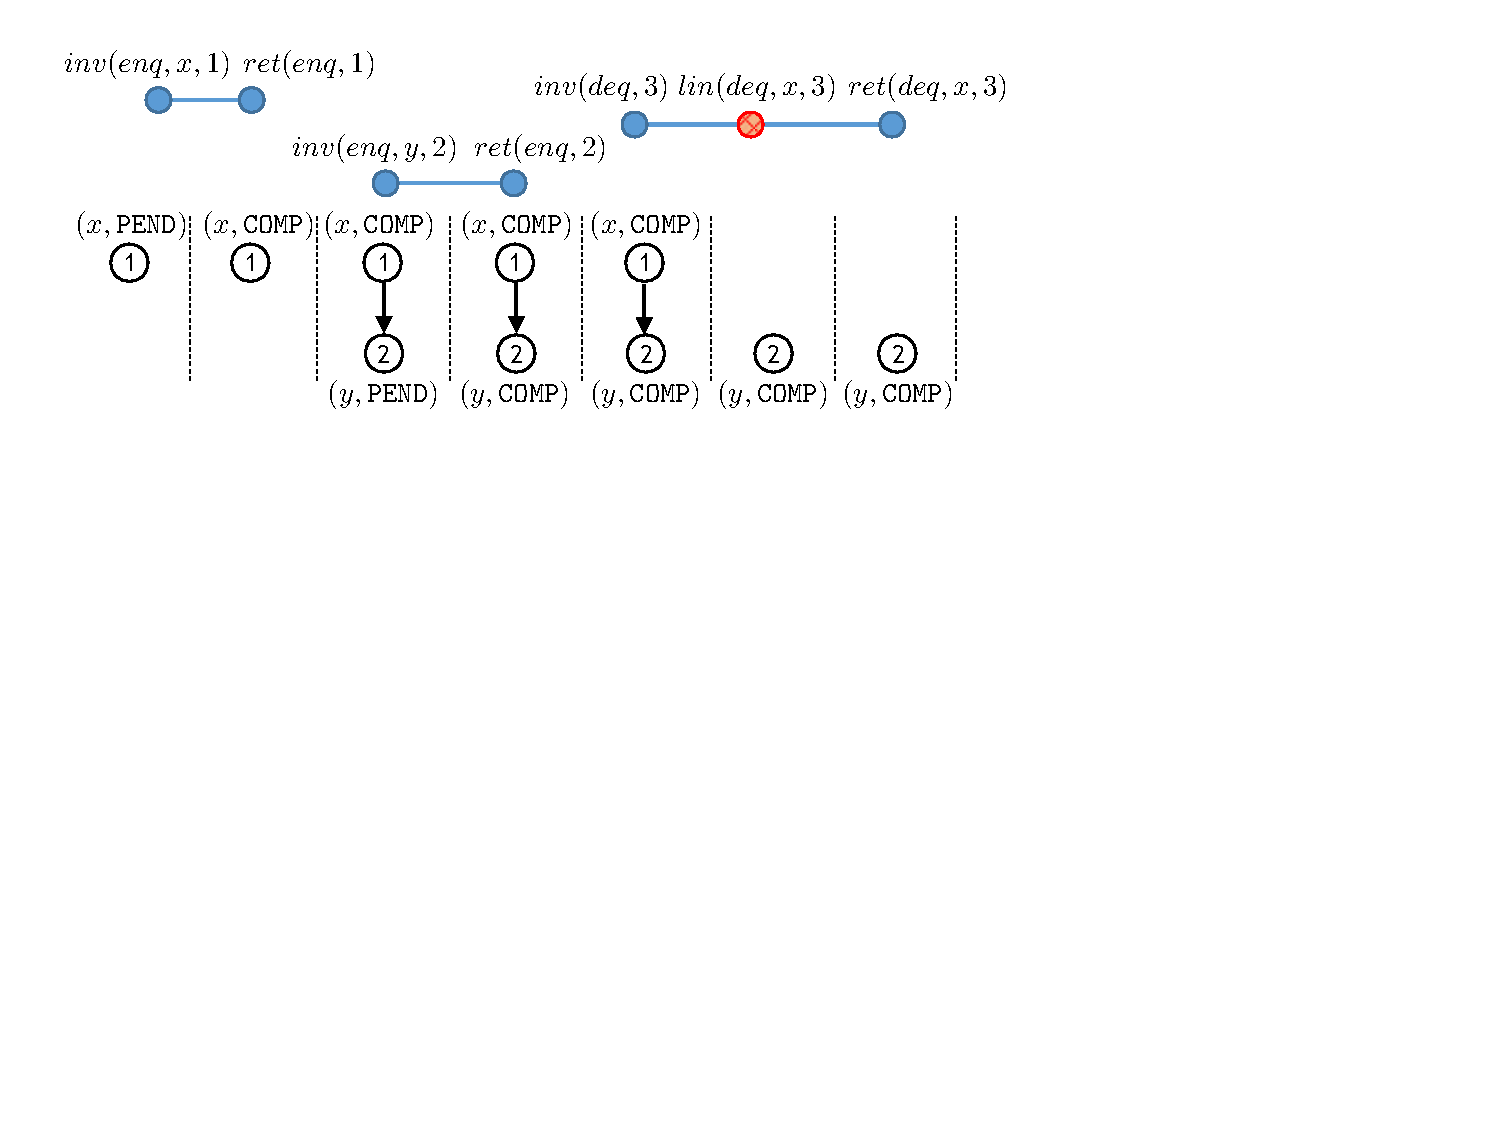
\includegraphics[width=7cm]{fig-queue2.pdf}
\begin{center}
(b)
\end{center}
\caption{Simulating queue histories with $AbsQ$.}
\label{fig:queueSim}
\end{wrapfigure}
SHOW HOW $AbsQ$ CAN SIMULATE SOME PROBLEMATIC HISTORIES

The states of $AbsQ$ are tuples $\tup{O,<,\ell,rv,cp}$ where $O\subseteq \<Ops>$ represents a set of operation identifiers (of previously invoked enqueue operations), $<\subseteq O\times O$ is a strict partial order, $\ell: O -> \<Vals>\times\{\tt{PEND,\tt{COMP}}\}$ labels every identifier with a value and a flag that records whether the operation is pending or completed (this flag is used to track the happens-before order), $rv:\<Ops> ~> \<Vals>$ records the return value of a pending dequeue fixed at its linearization point, and $cp:\<Ops> ~> \<Nats>$ records the control point of every pending (enqueue or dequeue) operation.
The initial state has all these components set to $\emptyset$ and the transition relation $->$ is defined in Figure~\ref{fig:transitions:AbsQ}. The alphabet of $AbsQ$ contains call/return actions and dequeue linearization points. The latter are denoted by $lin(deq,d,k)$ where $d\in \<Vals>$ and $k\in\<Ops>$. $Lin(deq)$ is the set of all such actions.

Concerning enqueue operations, the rule {\sc call-enq} orders the invoked operation after all the completed enqueue operations stored in the current state, and the rules {\sc ret-enq1}/{\sc ret-enq2} flip the corresponding flag from {\tt PEND} to {\tt COMP} provided that the operation is still present in the current state. For dequeue operations, {\sc call-deq} has no effect other than incrementing the control point and {\sc ret-deq} checks whether the return value is the same as the one fixed at the linearization point. The linearization point rule {\sc lin-deq1} corresponds to the case of a non-empty queue, showing that $lin(deq,d,k)$ is enabled only if the value $d$ has been added by an enqueue which is minimal in the current happens-before order. When it is enabled, it removes the enqueue adding $d$ from the state. The linearization point rule {\sc lin-deq2} corresponds to the case of dequeue operations linearized when the queue is empty.

\begin{figure} [t]
{\scriptsize
  \centering
  \begin{mathpar}
    \inferrule[call-enq]{
      k\not\in dom(cp) \\ 
    }{
      O,<,\ell,rv,cp
      \xrightarrow{inv(enq,d,k)}
      %O\cup\{k\},<\cup \{(k',k): \ell_2(k')={\tt COMP}\},\ell[k\mapsto (d,{\tt PEND})],rv,cp[k\mapsto 1]
      O\cup\{k\},<\cup\ {\tt COMP}(O)\times\{k\},\ell[k\mapsto (d,{\tt PEND})],rv,cp[k\mapsto 1]
    }\hspace{5mm}

    \inferrule[call-deq]{
      k\not\in dom(cp) \\ 
    }{
      O,<,\ell,rv,cp
      \xrightarrow{inv(deq,k)}
      O,<,\ell,rv,cp[k\mapsto 1]
    }\hspace{5mm}
    \inferrule[ret-deq]{
       cp(k) = 2 \\
       rv(k)=d  
    }{
      O,<,\ell,rv,cp
      \xrightarrow{ret(deq,d,k)}
      O,<,\ell,rv,cp[k\mapsto 3]
    }\hspace{5mm}

    \inferrule[ret-enq1]{
      cp(k) = 1 \\
      k \in O \\
      \ell(k) = (d,{\tt PEND}) 
    }{
      O,<,\ell,rv,cp
      \xrightarrow{ret(enq,k)}
      O,<,\ell[k\mapsto (d,{\tt COMP})],rv,cp[k\mapsto 2]
    }\hspace{5mm}
    \inferrule[ret-enq2]{
      cp(k) = 1 \\
      k \not\in O 
    }{
      O,<,\ell,rv,cp
      \xrightarrow{ret(enq,k)}
      O,<,\ell,rv,cp[k\mapsto 2]
    }\hspace{5mm}

    \inferrule[lin-deq1]{
       cp(k) = 1 \\
       d\neq{\tt EMPTY} \\
       k'\in min(O) \land \ell_1(k')=d
    }{
      O,<,\ell,rv,cp
      \xrightarrow{lin(deq,d,k)}
      O\setminus \{k'\},<\uparrow k',\ell,rv[k\mapsto d],cp[k\mapsto 2]
    }\hspace{5mm}

    \inferrule[lin-deq2]{
       cp(k) = 1 \\
       O=\emptyset
    }{
      O,<,\ell,rv,cp
      \xrightarrow{lin(deq,{\tt EMPTY},k)}
      O,<,\ell,rv[k\mapsto {\tt EMPTY}],cp[k\mapsto 2]
    }\hspace{5mm}

    
      \end{mathpar}
  }
 \vspace{-5mm}
  \caption{The transition relation of $AbsQ$. We use the following notations: $\ell_i(k)$ denotes the projection of $\ell(k)$ over the $i$-th component, for each $i\in\{1,2\}$, ${\tt COMP}(O)=\{k\in O: \ell_2(k)={\tt COMP}\}$, $\mathit{f}[x\mapsto y]$ is the function $g$ such that $g(z)=f(z)$ for all $z\neq x$ in the domain of $f$, and $g(x)=y$, $min(O)$ is the set of elements of $O$ which are minimal in the order relation $<$, and $<\uparrow k$ denotes the relation $<$ where all the pairs containing $k$ have been removed.}
  \label{fig:transitions:AbsQ}
\vspace{-6mm}
\end{figure}

Both methods have a fixed linearization point when the update of the shared sequence happens. Let $AbsQ_0$ denote this implementation~\footnote{For $\<Methods>=\{enq,deq\}$, the alphabet of $AbsQ_0$ is $C\cup R\cup Lin$.} (formally defined in Appendix~\ref{app:absImplQueue}).
The following result states that the library $AbsQ$ has exactly the same set of histories as the standard abstract library $AbsQ_0$ (see Appendix~\ref{app:absImplQueue} for a proof).

\begin{theorem}\label{th:absImplQueue}
$AbsQ$ is a refinement of $AbsQ_0$ and vice-versa.
\end{theorem}

A trace of a queue implementation is called \emph{$Lin(deq)$-complete} when every completed dequeue has a linearization point, i.e., TODO. A queue implementation $L$ over alphabet $\Sigma$ is called \emph{with fixed dequeue linearization points} if{f} $C\cup R\cup Lin(deq)\subseteq \Sigma$ 
and every trace $@t\in Tr(L)$ is $Lin(deq)$-complete.

TODO NEEDS DATA INDEPENDENCE FOR THE LINEARIZATION POINT TRANSITIONS TO BE DETERMINISTIC

The following result shows that $C\cup R\cup Lin(deq)$-forward simulations are a sound and complete proof method for showing the correctness of a queue implementation with fixed dequeue linearization points (up to the correctness of the linearization points). It is obtained from Theorem~\ref{th:absImplQueue} and Theorem~\ref{th:forSim} using the fact that the alphabet of $AbsQ$ is exactly $C\cup R\cup Lin(deq)$ and $AbsQ$ is deterministic.

\begin{corollary}
A queue implementation $L$ with fixed dequeue linearization points is a $C\cup R\cup Lin(deq)$-refinement of $AbsQ_0$ if{f} there exists a $C\cup R\cup Lin(deq)$-forward simulation from $L$ to $AbsQ$.
\end{corollary}

\subsection{A Correctness Proof For Herlihy\&Wing Queue}\label{ssec:HerlihyWing}
